\documentclass[a4paper]{article}
\usepackage{geometry}
\usepackage{graphicx}
\usepackage{natbib}
\usepackage{amsmath}
\usepackage{amssymb}
\usepackage{amsthm}
\usepackage{paralist}
\usepackage{epstopdf}
\usepackage{tabularx}
\usepackage{longtable}
\usepackage{multirow}
\usepackage{multicol}
\usepackage[hidelinks]{hyperref}
\usepackage{fancyvrb}
\usepackage{algorithm}
\usepackage{algorithmic}
\usepackage{float}
\usepackage{paralist}
\usepackage[svgname]{xcolor}
\usepackage{enumerate}
\usepackage{array}
\usepackage{times}
\usepackage{url}
\usepackage{fancyhdr}
\usepackage{comment}
\usepackage{environ}
\usepackage{times}
\usepackage{textcomp}
\usepackage{caption}
\usepackage{bbm}


\urlstyle{rm}

\setlength\parindent{0pt} % Removes all indentation from paragraphs
\theoremstyle{definition}
\newtheorem{definition}{Definition}[]
\newtheorem{conjecture}{Conjecture}[]
\newtheorem{example}{Example}[]
\newtheorem{theorem}{Theorem}[]
\newtheorem{lemma}{Lemma}
\newtheorem{proposition}{Proposition}
\newtheorem{corollary}{Corollary}

\floatname{algorithm}{Procedure}
\renewcommand{\algorithmicrequire}{\textbf{Input:}}
\renewcommand{\algorithmicensure}{\textbf{Output:}}
\newcommand{\abs}[1]{\lvert#1\rvert}
\newcommand{\norm}[1]{\lVert#1\rVert}
\newcommand{\RR}{\mathbb{R}}
\newcommand{\CC}{\mathbb{C}}
\newcommand{\Nat}{\mathbb{N}}
\newcommand{\br}[1]{\{#1\}}
\DeclareMathOperator*{\argmin}{arg\,min}
\DeclareMathOperator*{\argmax}{arg\,max}
\renewcommand{\qedsymbol}{$\blacksquare$}

\definecolor{dkgreen}{rgb}{0,0.6,0}
\definecolor{gray}{rgb}{0.5,0.5,0.5}
\definecolor{mauve}{rgb}{0.58,0,0.82}

\newcommand{\Var}{\mathrm{Var}}
\newcommand{\Cov}{\mathrm{Cov}}

\newcommand{\vc}[1]{\boldsymbol{#1}}
\newcommand{\xv}{\vc{x}}
\newcommand{\Sigmav}{\vc{\Sigma}}
\newcommand{\alphav}{\vc{\alpha}}
\newcommand{\muv}{\vc{\mu}}

\newcommand{\red}[1]{\textcolor{red}{#1}}

\def\x{\mathbf x}
\def\y{\mathbf y}
\def\w{\mathbf w}
\def\v{\mathbf v}
\def\E{\mathbb E}
\def\V{\mathbb V}
\def\ind{\mathbbm 1}

% TO SHOW SOLUTIONS, include following (else comment out):
\newenvironment{soln}{
    \leavevmode\color{blue}\ignorespaces
}{}


\hypersetup{
%    colorlinks,
    linkcolor={red!50!black},
    citecolor={blue!50!black},
    urlcolor={blue!80!black}
}

\geometry{
  top=1in,            % <-- you want to adjust this
  inner=1in,
  outer=1in,
  bottom=1in,
  headheight=3em,       % <-- and this
  headsep=2em,          % <-- and this
  footskip=3em,
}


\pagestyle{fancyplain}
\lhead{\fancyplain{}{Homework 5}}
\rhead{\fancyplain{}{CS 760 Machine Learning}}
\cfoot{\thepage}

\title{\textsc{Homework 5}} % Title

%%% NOTE:  Replace 'NAME HERE' etc., and delete any "\red{}" wrappers (so it won't show up as red)

\author{
$>>$Sean(Xiaoyu) Sun$<<$ \\
$>>$9078202463$<<$\\
} 

\date{}

\begin{document}

\maketitle 


\textbf{Instructions:} 
Although this is a programming homework, you only need to hand in a pdf answer file.
There is no need to submit the latex source or any code.
You can choose any programming language, as long as you implement the algorithm from scratch. 

Use this latex file as a template to develop your homework.
Submit your homework on time as a single pdf file to Canvas.
Please check Piazza for updates about the homework.



\section*{Linear Regression (100 pts total, 10 each)}

The Wisconsin State Climatology Office keeps a record on
the number of days Lake Mendota was covered by ice at
\url{http://www.aos.wisc.edu/~sco/lakes/Mendota-ice.html}.
Same for Lake Monona:
\url{http://www.aos.wisc.edu/~sco/lakes/Monona-ice.html}.
As with any real problems, the data is not as clean or as organized as one would like for machine learning.
Curate two clean data sets for each lake, respectively, starting from 1855-56 and ending in 2018-19.
Let $x$ be the year: for 1855-56, $x=1855$; for 2017-18, $x=2017$; and so on.
Let $y$ be the ice days in that year: for Mendota and 1855-56, $y=118$; for 2017-18, $y=94$; and so on.
Some years have multiple freeze thaw cycles such as 2001-02, that one should be $x=2001, y=21$.

\begin{enumerate}
\item
Plot year vs. ice days for the two lakes as two curves in the same plot.
Produce another plot for year vs. $y_{Monona} - y_{Mendota}$.

\begin{soln}
	   \begin{figure}[H]
	        \centering
	        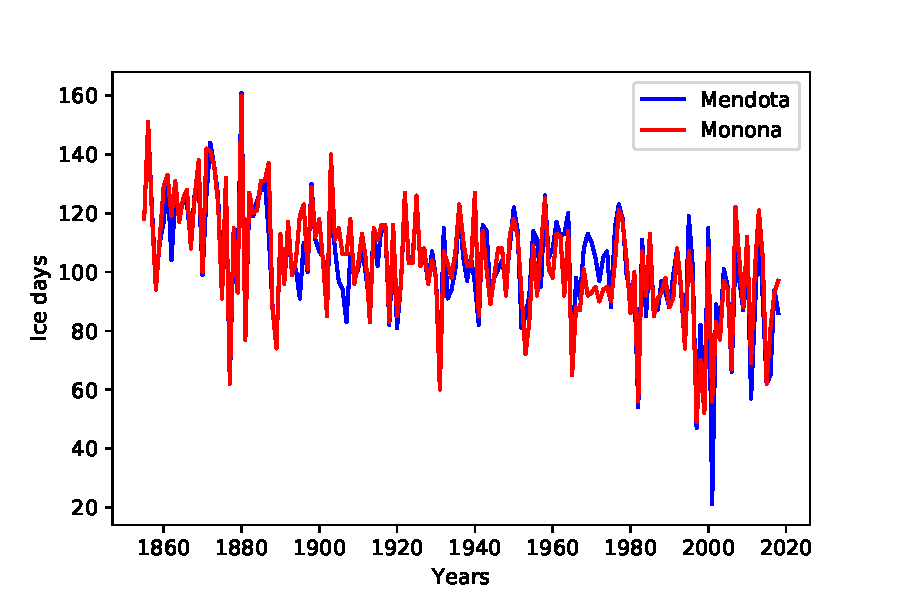
\includegraphics[width=0.5\textwidth]{q1_1.pdf}
	        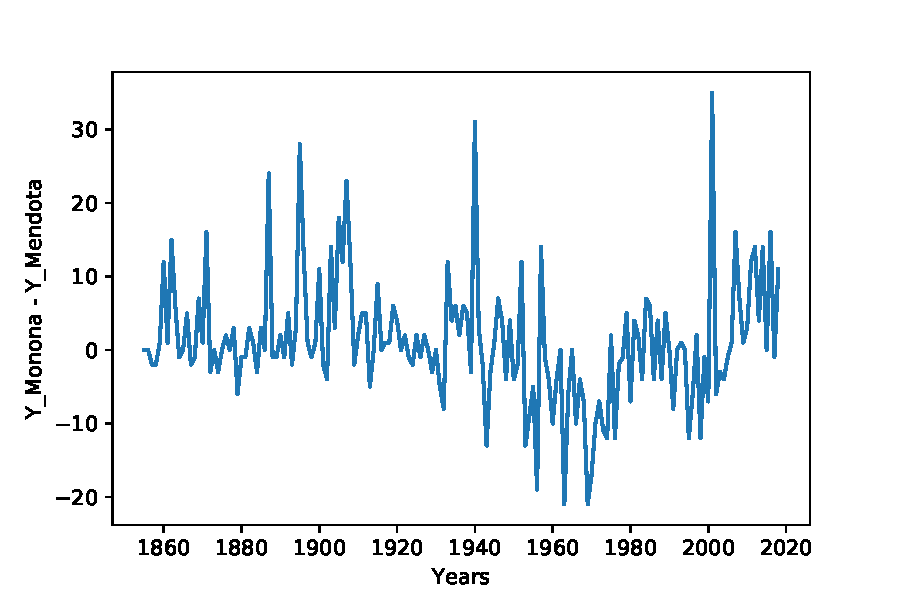
\includegraphics[width=0.5\textwidth]{q1_2.pdf}
	        \captionsetup{labelformat=empty}
	        \caption{}
	        \label{fig:my_label}
	   \end{figure}

\end{soln}

\item
Split the datasets: $x\le 1970$ as training, and $x>1970$ as test.
(Comment: due to the temporal nature this is NOT an iid split.  But we will work with it.)
On the training set, compute the sample mean $\bar y=\frac{1}{n}\sum_{i=1}^n y_i$ and the sample standard deviation $\sqrt{\frac{1}{n-1}\sum_{i=1}^n (y_i-\bar y)^2}$ for the two lakes, respectively.

\begin{soln}
Mendota:\\
  mean:  107.1896551724138\\
  std:  16.74666159754441\\
Monona:\\
  mean:  108.48275862068965\\
  std:  18.122521543826256\\
\end{soln}

\item
Using training sets, train a linear regression model
$$\hat y_{Mendota} = \beta_0 + \beta_1 x + \beta_2 y_{Monona}$$
to predict $y_{Mendota}$.
Note: we are treating $y_{Monona}$ as an observed feature.
Do this by finding the closed-form MLE solution for $\beta=(\beta_0, \beta_1, \beta_2)^\top$ (no regularization):
$$\min_\beta {1\over n} \sum_{i=1}^n (x_i^\top \beta - y_i)^2.$$
Give the MLE formula in matrix form (define your matrices), then give the MLE value of $\beta_0, \beta_1, \beta_2$. 

\begin{soln}
Formula: $\beta_{MLE} =  (X^TX)^{-1}X^TY$\\
where 

$$  
X =
\begin{bmatrix}
   1 & year_1 & days_1 \\
   ...& ... & ... \\
   1 & year_{n} & days_{n} 
 \end{bmatrix} $$ 
and $year_i$ and $days_i$ are $i^{th}$ year in the record and the corresponding Monona ice days in that year\\
$Y$ is the $n\times 1$ matrix recording ice days for every year\\
The result of $\beta$ is $[-64.182766, 0.041225, 0.852951]$

\end{soln} 


\item
Using the MLE above, give the (1) mean squared error and (2) $R^2$ values on the Mendota test set.
(You will need to use the Monona test data as observed features.)


\begin{soln}
MSE = 124.26409483979052\\ 
$R^{2}$ = 0.7104900715614509
\end{soln}

\item
``Reset'' to Q3, but this time use gradient descent to learn the $\beta$'s.
Recall our objective function is the mean squared error on the training set:
$${1\over n} \sum_{i=1}^n (x_i^\top \beta - y_i)^2.$$
Derive the gradient.

\begin{soln}
$\nabla_{\beta}({1\over n} \sum_{i=1}^n (x_i^\top \beta - y_i)^2) \\\\= \frac{\partial ({1\over n} \sum_{i=1}^n (x_i^\top \beta - y_i)^2)}{\partial \beta} \\= \frac{\partial (\frac{1}{n}(X\beta - Y)^T(X\beta - Y))}{\partial \beta}\\= \frac{2}{n}X^T(X\beta - Y)$
\end{soln}

\item
Implement gradient descent.  Initialize $\beta_0= \beta_1= \beta_2=0$.  Use a fixed stepsize parameter $\eta=0.1$ and print the first 10 iteration's objective function value.
Tell us if further iterations make your gradient descent converge, and if yes when; compare the $\beta$'s to the closed-form solution.
Try other $\eta$ values and tell us what happens.
\textbf{Hint:} Update $\beta_0, \beta_1, \beta_2$ simultaneously in an iteration.  Don't use a new $\beta_0$ to calculate $\beta_1$, and so on.

\begin{soln}
epoch 1:  6180350808297761.0\\
epoch 2:  3.330626781514358e+27\\
epoch 3:  1.7948940285065868e+39\\
epoch 4:  9.672787691041719e+50\\
epoch 5:  5.212721209720432e+62\\
epoch 6:  2.8091655971560845e+74\\
epoch 7:  1.5138755814390704e+86\\
epoch 8:  8.158363032772628e+97\\
epoch 9:  4.396589005764993e+109\\
epoch 10:  2.3693472339933727e+121\\

This shows that setting learning rate to be 0.1 doesn't make it converge and those loss are much larger than the loss gotten from using closed-form method.
Obviously, this is because the learning rate (step size) is too big. After I tried different step sizes, I found that when $\eta = 1e-7$, the loss decreased in a much faster rate and converged. What's interesting is that when $\eta = 1e-8$, the decreasing rate became slower than 1e-7. So we should be careful about choosing learning rate or step size.

\end{soln}


\item
As preprocessing, normalize your year and Monona features (but not $y_{Mendota}$).
Then repeat Q6.

\begin{soln}
epoch 1:  7545.998373501812\\
epoch 2:  4850.273518530398\\
epoch 3:  3127.473895121937\\
epoch 4:  2025.60791967957\\
epoch 5:  1320.3620154290256\\
epoch 6:  868.6443341670556\\
epoch 7:  579.0974806545669\\
epoch 8:  393.3511885316234\\
epoch 9:  274.0870881867737\\
epoch 10:  197.4318389691094\\
\end{soln}

\item 
``Reset'' to Q3 (no normalization,  use closed-form solution), but train a linear regression model without using Monona:
$$\hat y_{Mendota} = \gamma_0 + \gamma_1 x.$$
  \begin{enumerate}
  \item Interpret the sign of $\gamma_1$.
  \item Some analysts claim that because $\beta_1$ the closed-form solution in Q3 is positive, fixing all other factors, as the years go by the number of Mendota ice days will increase, namely the model in Q3 indicates a cooling trend. Discuss this viewpoint, relate it to question 8(a).
  \end{enumerate}

\begin{soln}
(a).\\
 $\gamma_0 = 406.111060, \gamma_1 =  -0.156299$\\
 The sign of $\gamma_1$ is negative, which means with the increase of year, the icy days decreases. Contrary to Q3, this indicates a warming trend.

(b).\\
I think this viewpoint is untenable. In Q3, we have another feature, namely the ice days of Monona. Though $\beta_1$, which is the parameter for year feature in Q3, is positve, we can notice that $\beta_2$, which is the parameter for ice days of Monona, is also postive and is relatively much larger than $\beta_1$. From the plot in Q1 we can notice that Monona ice days has a decreasing trend. So, model from Q3 actually also predicted a warming trend since it learned a larger parameter for decreasing feature and relatively smaller parameter for increasing feature. This result is consistent with (a).
\end{soln}

\item
Of course, Weka has linear regression.  Reset to Q3.  Save the training data in .arff format for Weka.  Use classifiers / functions / LinearRegression.  Choose ``Use training set.''  
  Bring up Linear Regression options, set ``ridge'' to 0 so it does not regularize.  Run it and tell us the model: it is in the output in the form of ``$\beta_1$ * year + $\beta_2$ * Monona + $\beta_0$.'' 

\begin{soln}
$days = 0.0412 * years + 0.853  * monona -64.1828$
\end{soln}

\item Ridge regression.
\begin{enumerate}
\item
Then set ridge to 1 and tell us the resulting Weka model.

\begin{soln}
$days = 0.0387 * years + 0.8436 * monona -58.3961$
\end{soln}
\item
Meanwhile, derive the closed-form solution in matrix form for the ridge regression problem:
$$\min_\beta \left({1\over n} \sum_{i=1}^n (x_i^\top \beta - y_i)^2 \right) + \lambda \|\beta\|_A^2$$
where 
$$\|\beta\|_A^2 := \beta^\top A \beta$$
and
$$A=
\begin{bmatrix}
0 & 0 & 0 \\
0 & 1 & 0 \\
0 & 0 & 1
\end{bmatrix}.$$
This $A$ matrix has the effect of NOT regularizing the bias $\beta_0$, which is standard practice in ridge regression.
Note: Derive the closed-form solution, do not blindly copy lecture notes.

\begin{soln}
$Loss = \frac{1}{n} \times(X\beta - Y)^T(X\beta - Y) + \lambda (\beta^T A \beta) $\\
$\frac{\partial Loss}{\partial \beta} =\frac{1}{n} \times 2X^T(X\beta - Y)+2 \lambda A\beta = 0$\\
$(X^TX\beta +n\lambda A \beta) - X^TY = 0$\\\\
$ \beta = (X^TX +n\lambda A)^{-1}X^TY$
\end{soln}
\item
Let $\lambda=1$ and tell us the value of $\beta$ from your ridge regression model.

\begin{soln}
$\beta = [-62.329472, 0.040439, 0.849715]$
\end{soln}

\end{enumerate}

\end{enumerate}

\end{document}
\bibliographystyle{apalike}
\end{document}
